% ========================================= TEMPLATE INFO ========================================
%
% Author:       P4ntomime
% Version:      1.0.0
% Last updated: 2024-02-18
% Brief:        A LaTeX template for summaries. See README.md for more information.
% 
% ================================================================================================
\documentclass[8pt, a4paper, twoside, landscape]{extarticle}
% Font size:    8pt
% Paper size:   A4
% style:        twoside (needed, so odd and even pages have different margins)
% orientation:  portrait. (use 'landscape' for landscape orientation)


% ========================================= DOCUMENT INFO =========================================
\def\title{Volkswirtschaftslehre}       % title
\def\shorttitle{Volkswirtschaftslehre}                            % short title (displayed as PDF title)
\def\dozent{Dr. Daniel Alberer}               % docent
\def\semester{FS 2026}                              % semester
\def\author{Gian Marco Näf}                           % author(s)
\def\repo{https://github.com/Giamo08/Zusammenfassungen}        % repository link
\def\version{3.0.\today}                            % version
\def\pagelimit{50}                                   % page limit -> causes pages after limit to be red
\def\titleoption{ultra compact}                     % options: ultra compact, compact, normal
\def\enableToC{false}

% ================================= PACKAGES, SETUP AND COMMANDS ==================================
\makeatletter
\def\input@path{{./}{VwlWp/}}
\makeatother
\input{preamble.tex}
\makeatletter
\def\@enableToC{true}
\ifx\enableToC\@enableToC
    \setcounter{tocdepth}{2} % adjust depth: 0=parts,1=sections,2=subsections,...
    \AtBeginDocument{%
        \clearpage
        \tableofcontents
        \clearpage
    }s
\fi
\makeatother

% =========================================== DOCUMENT ============================================
\begin{document}
    \begin{layout}
        \section{Wohlstand}

\subsection{Einordnung und Zielsetzung der Volkswirtschaftslehre}

Die Volkswirtschaftslehre beschäftigt sich mit der Frage, wie eine Gesellschaft 
mit ihren knappen Ressourcen umgeht. Zu diesen Ressourcen zählen insbesondere 
Arbeit, Kapital, Technologie, Boden sowie natürliche Ressourcen. 

Sie gliedert sich in drei zentrale Bereiche:

\begin{itemize}
    \item \textbf{Mikroökonomie:} Analyse der Entscheidungen einzelner Wirtschaftseinheiten 
    (Haushalte, Unternehmen, Staat, Ausland).
    \item \textbf{Makroökonomie:} Untersuchung der gesamtwirtschaftlichen Zusammenhänge 
    und der Koordination dieser Einzelentscheidungen.
    \item \textbf{Wirtschaftspolitik:} Ableitung wirtschaftspolitischer Massnahmen im 
    Hinblick auf Wachstum, Beschäftigung, Inflation und Innovation.
\end{itemize}

Ziel der ersten Lerneinheit ist es, den Begriff \textit{Wohlstand} zu definieren, 
seine Entstehung zu erklären und seine Messung kritisch zu reflektieren.

\subsection{Ziele der Wirtschaftspolitik}

\begin{center}
    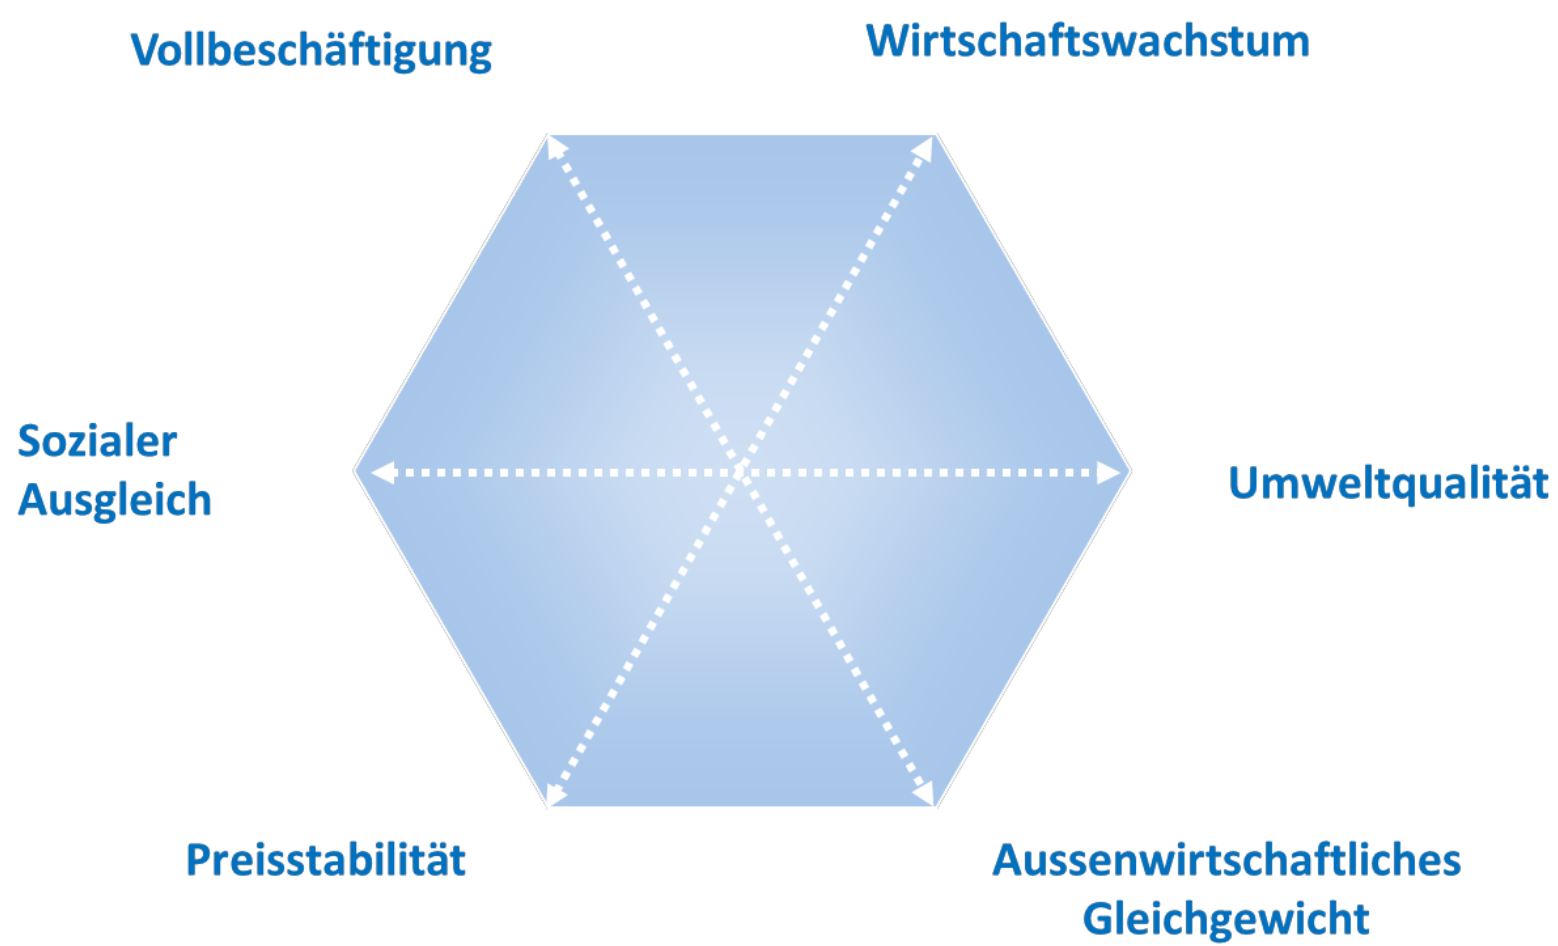
\includegraphics[width=0.8\linewidth]{images/hexagon.png}
\end{center}
Die Wirtschaftspolitik verfolgt mehrere Zielsetzungen, die häufig in einem 
Zielpolygon dargestellt werden:

\begin{itemize}
    \item Vollbeschäftigung
    \item Wirtschaftswachstum
    \item Preisstabilität
    \item Sozialer Ausgleich
    \item Umweltqualität
    \item Aussenwirtschaftliches Gleichgewicht
\end{itemize}

Zwischen diesen Zielen bestehen unterschiedliche Beziehungen:

\begin{itemize}
    \item \textbf{Zielharmonie:} Zwei Ziele unterstützen sich gegenseitig.
    \item \textbf{Zielneutralität:} Zwei Ziele beeinflussen sich nicht.
    \item \textbf{Zielkonflikt (Trade-off):} Die Erreichung eines Ziels erschwert 
    die Erreichung eines anderen.
\end{itemize}

Die Wirtschaftspolitik steht somit vor der Aufgabe, Zielkonflikte abzuwägen.

\subsection{Akteure der Volkswirtschaft und Wirtschaftskreislauf}

\begin{center}
    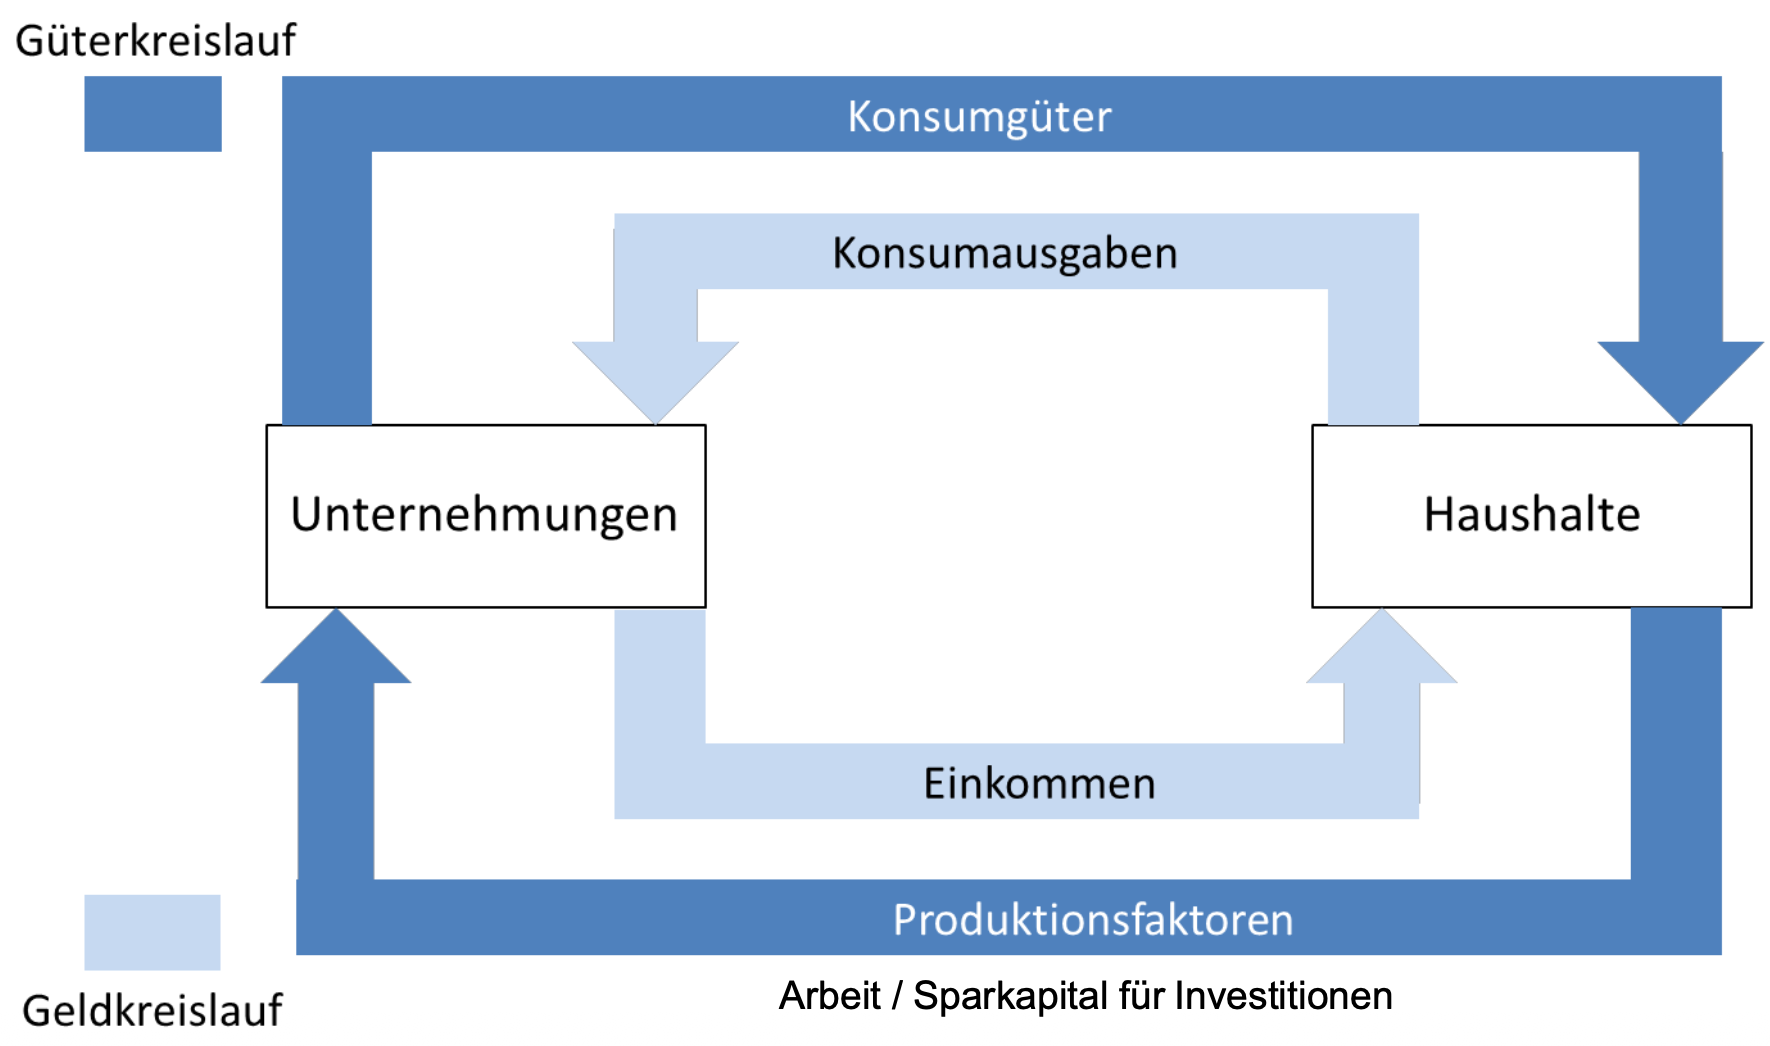
\includegraphics[width=0.8\linewidth]{images/kreislaufGueter.png}
\end{center}
\begin{center}
    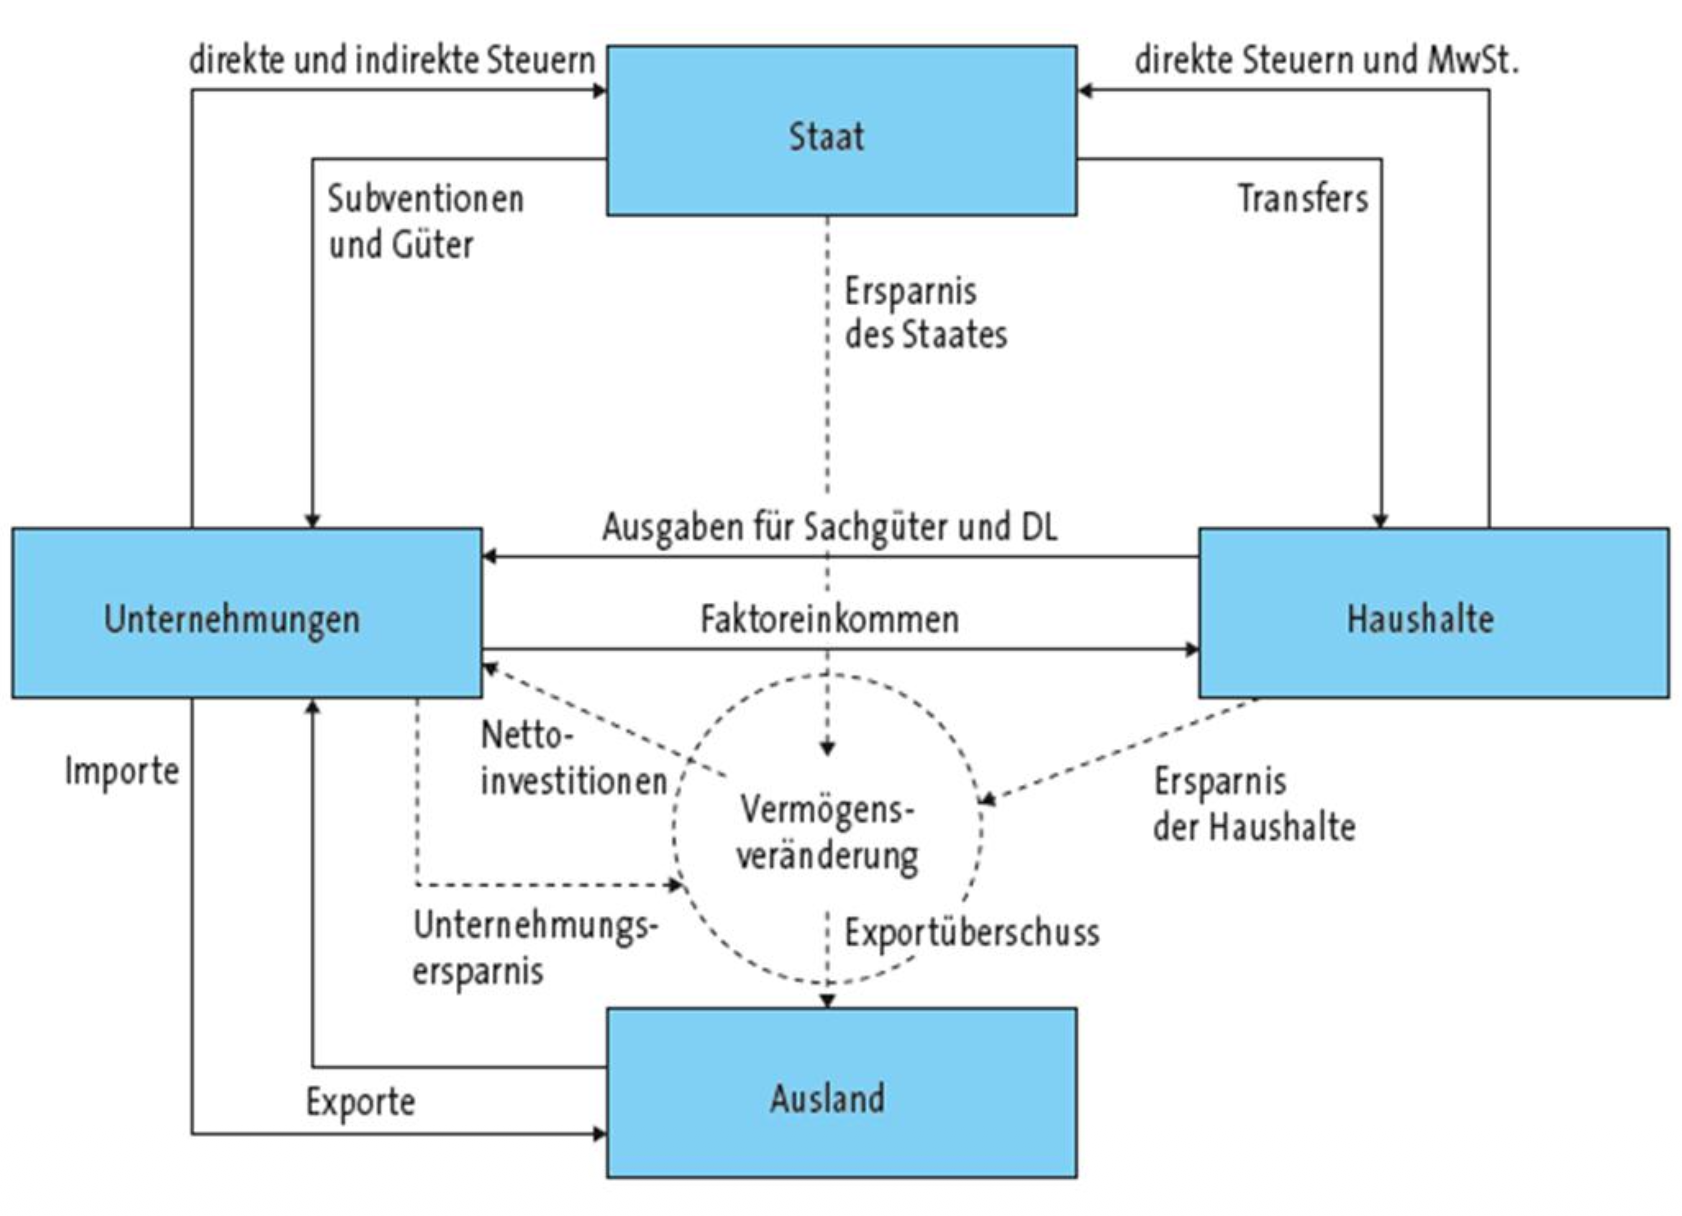
\includegraphics[width=0.8\linewidth]{images/erweiterterKreislauf.png}
\end{center}

Die Volkswirtschaft besteht aus vier zentralen Akteuren:

\begin{itemize}
    \item Haushalte
    \item Unternehmen
    \item Staat
    \item Ausland
\end{itemize}

Im einfachen Wirtschaftskreislauf stellen Haushalte Produktionsfaktoren 
(insbesondere Arbeit) zur Verfügung und erhalten Einkommen. Unternehmen 
produzieren Güter und zahlen Löhne sowie Gewinne.

Im erweiterten Wirtschaftskreislauf treten zusätzlich Staat und Ausland auf. 
Der Staat erhebt Steuern, zahlt Transfers und tätigt Ausgaben. 
Das Ausland beeinflusst die Volkswirtschaft über Exporte und Importe.

Diese Kreisläufe zeigen, dass Produktion, Einkommen und Verwendung 
eng miteinander verknüpft sind.

\subsection{Definition von Wohlstand}

Wohlstand wird definiert als Grad der Versorgung von Personen, Haushalten 
oder der gesamten Gesellschaft mit Gütern.

Wohlstand ist somit primär ein materielles Konzept und bezieht sich auf 
die Verfügbarkeit wirtschaftlicher Güter und Dienstleistungen.

\subsection{Messung des Wohlstands: Das Bruttoinlandprodukt (BIP)}

In der Praxis wird Wohlstand meist über das Bruttoinlandprodukt (BIP) gemessen.

Das BIP entspricht dem Wert aller in einem Land während eines Jahres 
produzierten und nachgefragten Güter und Dienstleistungen abzüglich 
der Vorleistungen. 

Formal entspricht es der \textbf{Wertschöpfung}.

Dabei gilt:

\[
BIP = Produktionswert - Vorleistungen + Gütersteuern - Gütersubventionen
\]

Wichtig ist, dass das BIP nur marktfähige, bezahlte Leistungen erfasst. 
Nicht entlöhnte Tätigkeiten wie Hausarbeit oder informelle Leistungen 
werden nicht berücksichtigt.

\subsection{Nominales und reales BIP}

Es wird unterschieden zwischen:

\begin{itemize}
    \item \textbf{Nominalem BIP:} Bewertung zu laufenden Preisen.
    \item \textbf{Realem BIP:} Preisbereinigte Darstellung, um Inflationseffekte 
    auszuschliessen.
    \item \textbf{BIP pro Kopf:} Durchschnittlicher Wohlstand pro Einwohner.
    \item \textbf{Kaufkraftbereinigtes BIP:} Internationale Vergleichbarkeit 
    unter Berücksichtigung unterschiedlicher Preisniveaus.
\end{itemize}

Das reale BIP pro Kopf gilt als zentrale Kennzahl zur Beurteilung 
des langfristigen Wohlstandsniveaus.

\subsection{Die drei Perspektiven der Volkswirtschaftlichen Gesamtrechnung (VGR)}

\begin{center}
    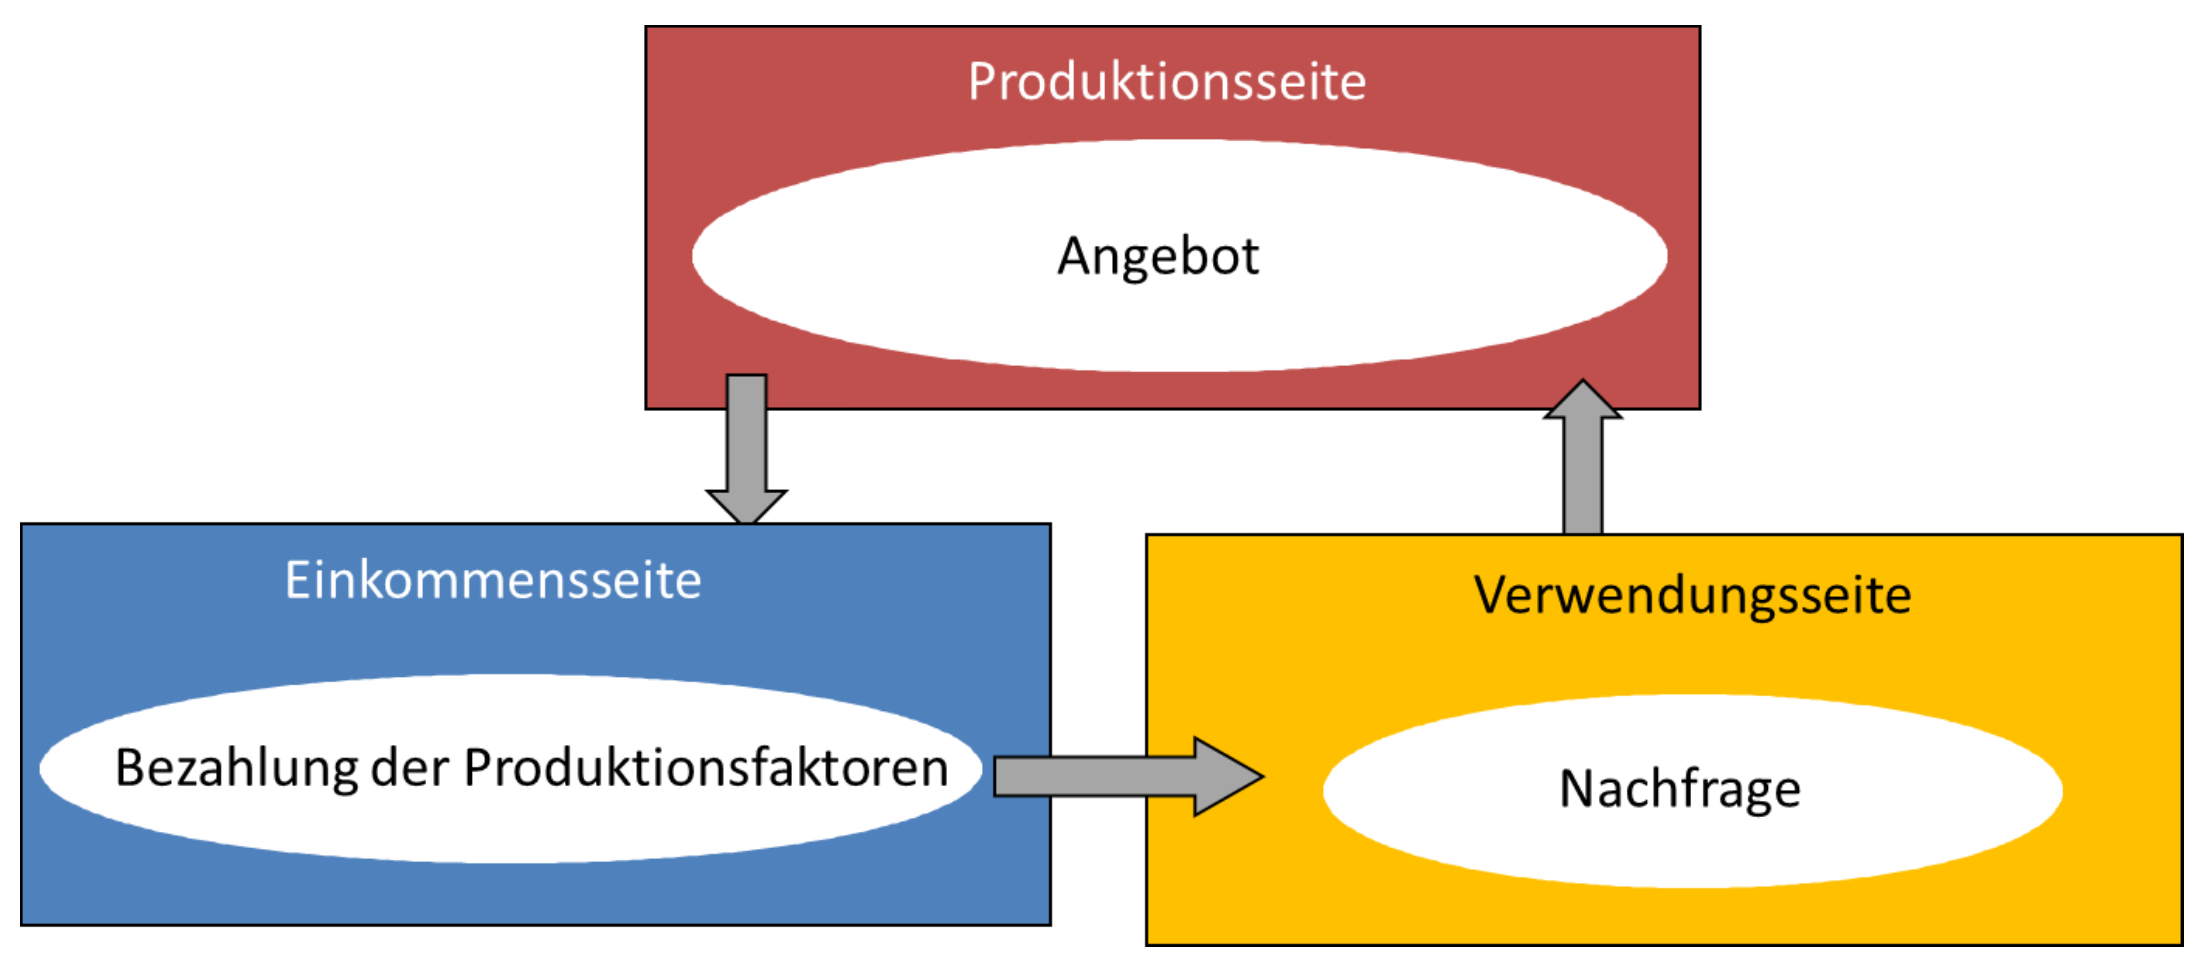
\includegraphics[width=0.8\linewidth]{images/vgr3blickwinkel.png}
\end{center}

Das BIP kann aus drei Blickwinkeln berechnet werden:

\begin{enumerate}
    \item \textbf{Produktionsseite:} Summe der Wertschöpfung aller Branchen.
    \item \textbf{Verwendungsseite:} Summe aus Konsum, Investitionen, 
    Staatsausgaben und Nettoexporten.
    \item \textbf{Einkommensseite:} Summe der Einkommen (Löhne, Gewinne, 
    Abschreibungen, Steuern minus Subventionen).
\end{enumerate}

Alle drei Ansätze führen zum gleichen BIP-Wert.

\subsection{Struktur der Schweizer Wertschöpfung}

Die Produktionsseite zeigt, welche Branchen besonders zur Wertschöpfung 
beitragen. In der Schweiz haben insbesondere folgende Sektoren ein hohes Gewicht:

\begin{itemize}
    \item Grosshandel
    \item Öffentliche Verwaltung
    \item Gesundheitswesen
    \item Finanzdienstleistungen und Versicherungen
    \item Pharmaindustrie
\end{itemize}

Die Struktur der Wirtschaft beeinflusst somit die Stabilität und das 
Wachstumspotenzial eines Landes.

\subsection{Internationale Wohlstandsvergleiche}

Beim Vergleich von Ländern ist zwischen absolutem BIP und BIP pro Kopf 
zu unterscheiden.

Ein Land kann ein hohes Gesamt-BIP aufweisen (z.\,B. USA oder China), 
ohne dass der durchschnittliche Wohlstand pro Person besonders hoch ist.

Das BIP pro Kopf erlaubt eine bessere Einschätzung des individuellen 
materiellen Wohlstands.

\subsection{Grenzen der Volkswirtschaftlichen Gesamtrechnung}

Die VGR weist mehrere Schwächen auf:

\begin{itemize}
    \item Nicht erfasste Tätigkeiten (z.\,B. unbezahlte Arbeit)
    \item Schwarzarbeit und informelle Wirtschaft
    \item Fehlende Marktpreise für öffentliche Güter
    \item Keine Aussage über Einkommensverteilung
\end{itemize}

Das BIP misst daher nur einen Teil des tatsächlichen Wohlstands.

\subsection{Wohlstand und Lebensqualität}

Wohlstand ist nicht gleichbedeutend mit Lebensqualität.

Lebensqualität umfasst zusätzliche Dimensionen wie:

\begin{itemize}
    \item Gesundheit
    \item Bildung
    \item Sicherheit
    \item Umweltqualität
    \item soziale Beziehungen
    \item politische Rechte
\end{itemize}

Ein Beispiel für einen erweiterten Ansatz ist der \textbf{Social Progress Index (SPI)}. 
Dieser misst soziale Entwicklung anhand von 54 Indikatoren, die in drei Hauptkategorien 
zusammengefasst werden:

\begin{itemize}
    \item Basic Human Needs
    \item Foundations of Wellbeing
    \item Opportunity
\end{itemize}

Empirisch besteht zwar eine positive Korrelation zwischen BIP und sozialem Fortschritt, 
doch steigt die Lebensqualität ab einem bestimmten Einkommensniveau weniger stark an.

\subsection{Zusammenfassung}

Wohlstand bezeichnet die materielle Versorgung einer Gesellschaft mit Gütern 
und wird in der Regel durch das BIP gemessen. 

Das BIP kann aus Produktions-, Verwendungs- und Einkommensperspektive 
ermittelt werden. 

Trotz seiner Bedeutung weist es konzeptionelle Grenzen auf und erfasst 
nicht alle Dimensionen gesellschaftlichen Wohlergehens. 

Für eine umfassende Beurteilung des gesellschaftlichen Fortschritts 
müssen daher zusätzliche Indikatoren der Lebensqualität berücksichtigt werden.
        \section{ Wirtschaftswachstum}

\subsection{Problemstellung: Warum Wachstum?}

Wenn Wohlstand positiv mit Lebensqualität korreliert, stellt sich die strategische Frage:

\begin{itemize}
    \item Wie kann langfristiger Wohlstand gesteigert werden?
    \item Welche Wachstumsquellen sind politisch beeinflussbar?
    \item Wie entwickelte sich das BIP pro Kopf der Schweiz?
    \item Warum wurde 2004 eine offizielle Wachstumspolitik eingeführt?
\end{itemize}

Wachstum ist im Zielpolygon der Wirtschaftspolitik zentral verankert.

\subsection{Bedeutung des langfristigen Wachstums}

\begin{center}
    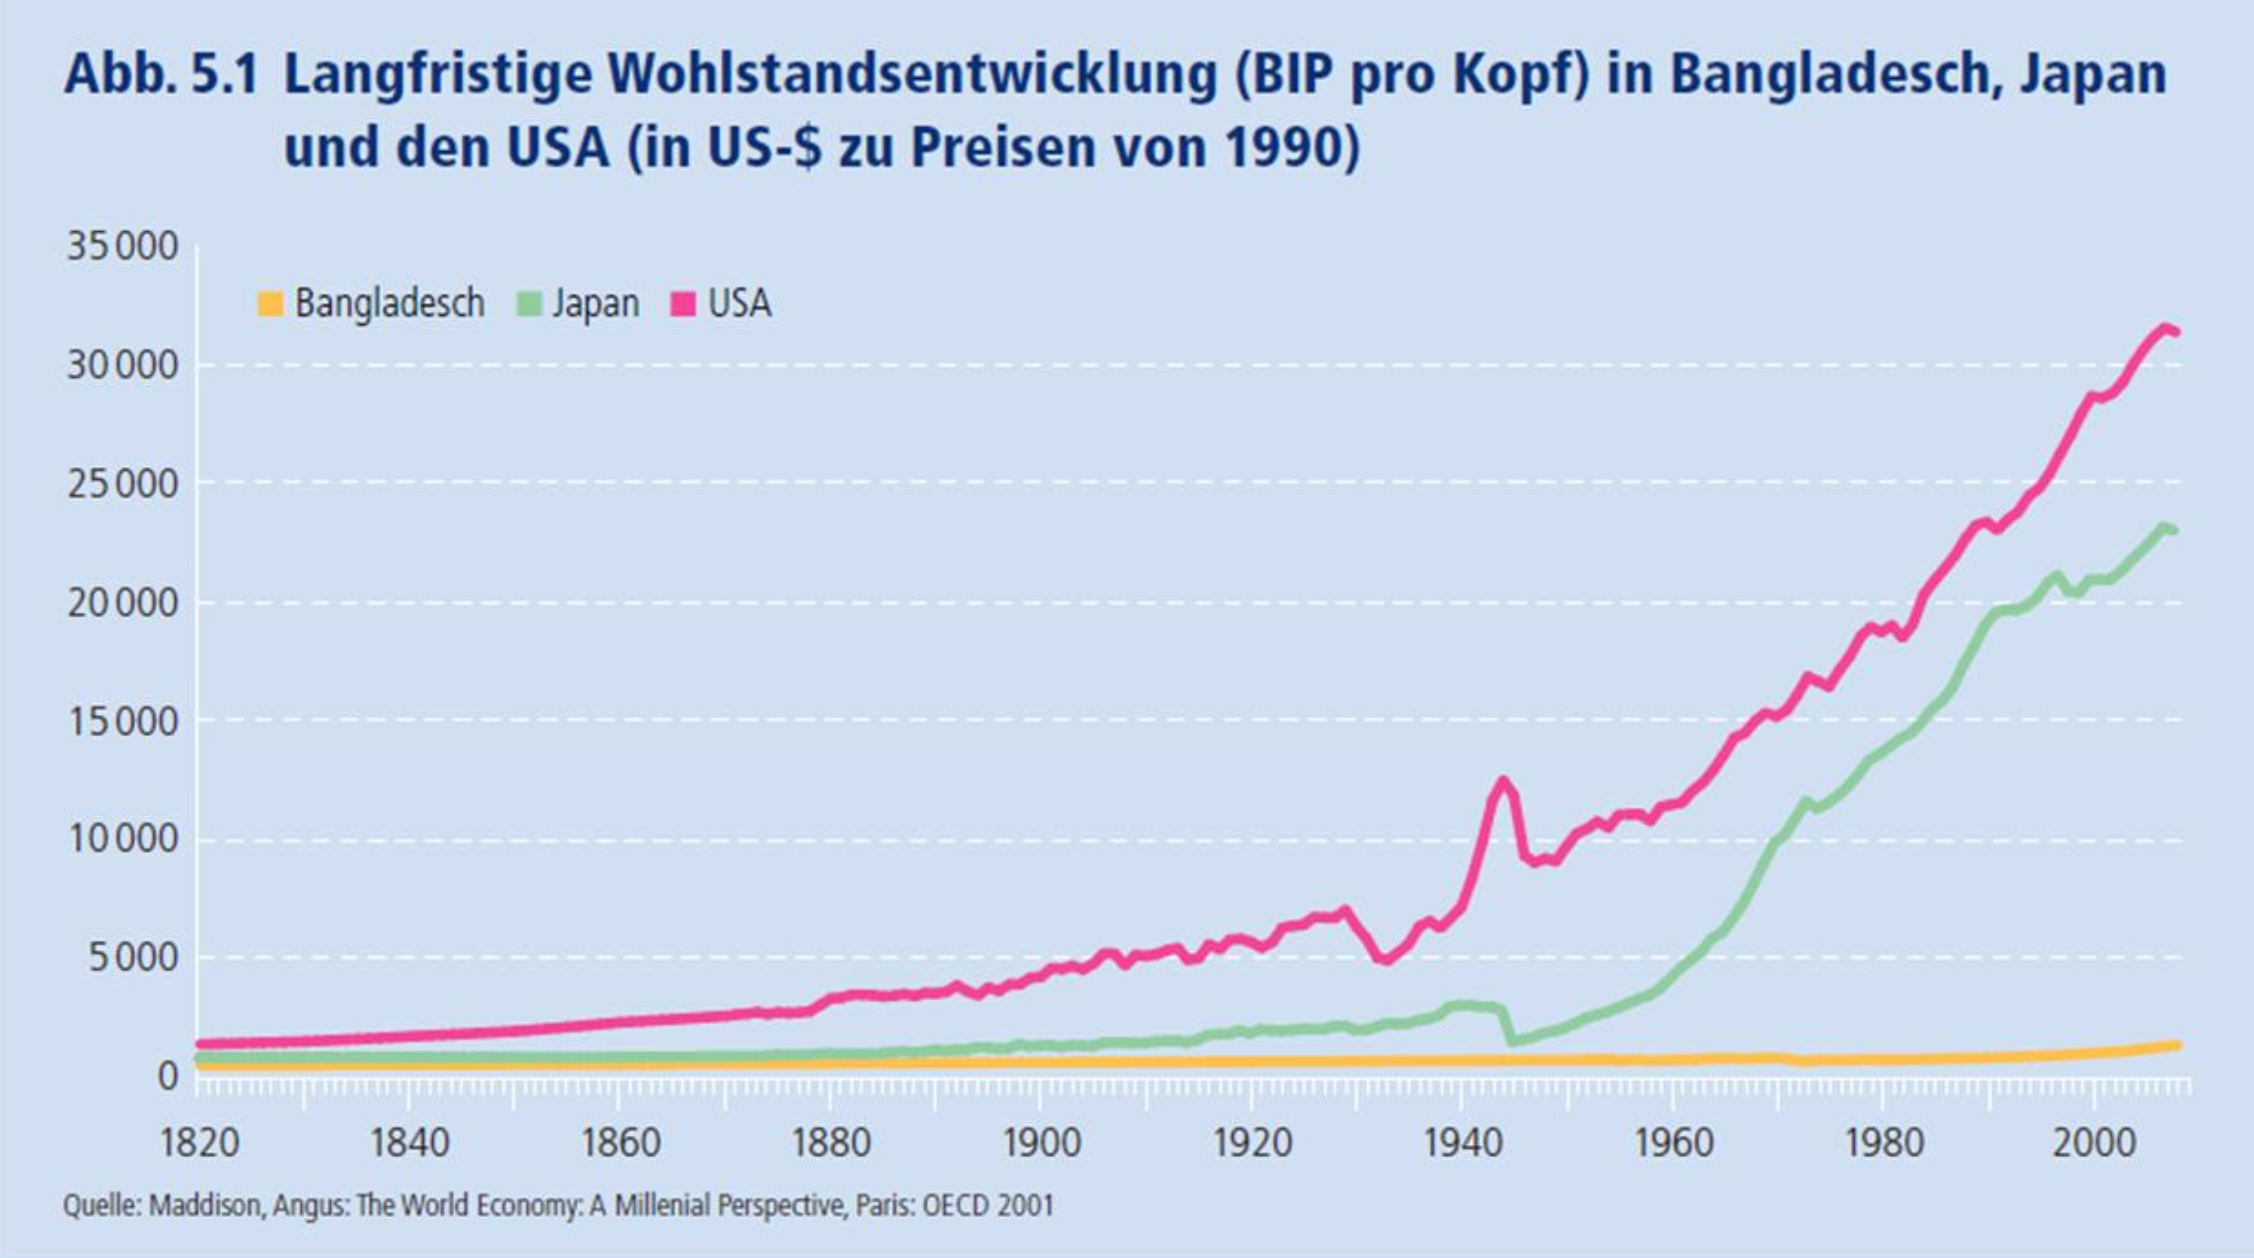
\includegraphics[width=0.8\linewidth]{images/bip_pro_Kopf.png}
\end{center}

Langfristige Unterschiede im Wachstum führen zu massiven Wohlstandsdifferenzen.

Empirischer Vergleich (Bangladesch, Japan, USA):
Kleine Wachstumsunterschiede kumulieren sich exponentiell.

Wachstum erleichtert Verteilung:
Neu geschaffener Wohlstand lässt sich politisch einfacher verteilen als bestehender umzuverteilen.

\subsection{Wachstum vs. Konjunktur}

Unterscheidung:

\begin{itemize}
    \item \textbf{Wachstumstrend:} langfristige Entwicklung des Produktionspotenzials
    \item \textbf{Konjunktur:} kurzfristige Schwankungen um den Trend
\end{itemize}

Konjunktur führt zu Unter- oder Überauslastung.
Langfristiger Wohlstand hängt vom Trend ab, nicht von kurzfristigen Zyklen.

\subsection{Quellen des Wachstums}

\begin{center}
    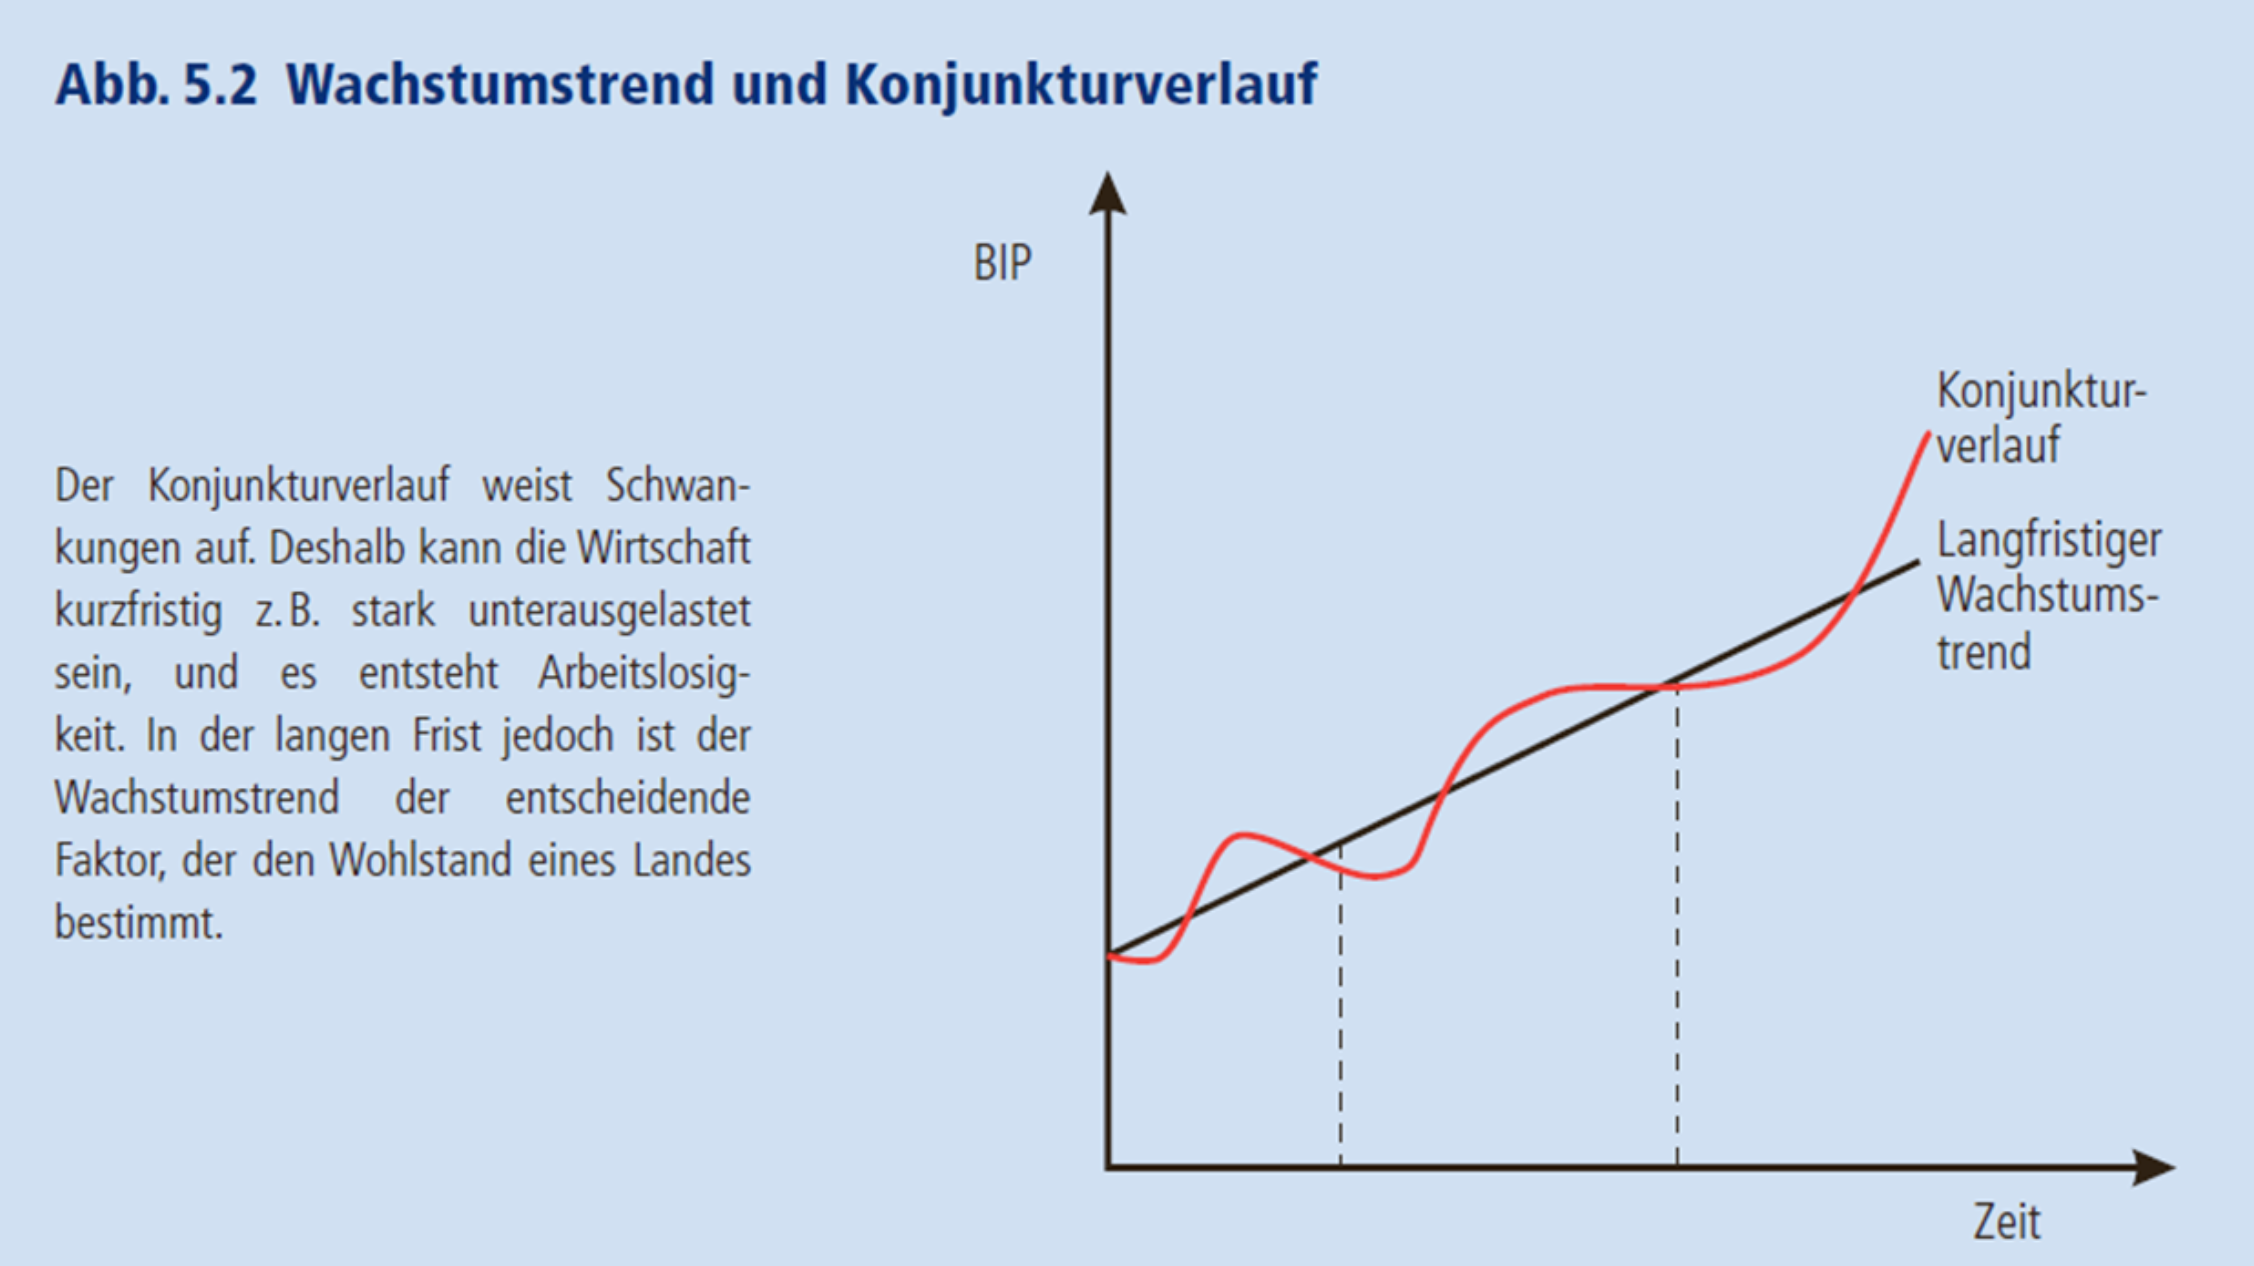
\includegraphics[width=0.8\linewidth]{images/wachstumstrend_konjunkturverlauf.png}
\end{center}

Wachstum des BIP pro Kopf entsteht durch:

\begin{enumerate}
    \item Mehr Arbeitsstunden
    \item Höhere Produktion pro Arbeitsstunde (Arbeitsproduktivität)
\end{enumerate}

\begin{center}
    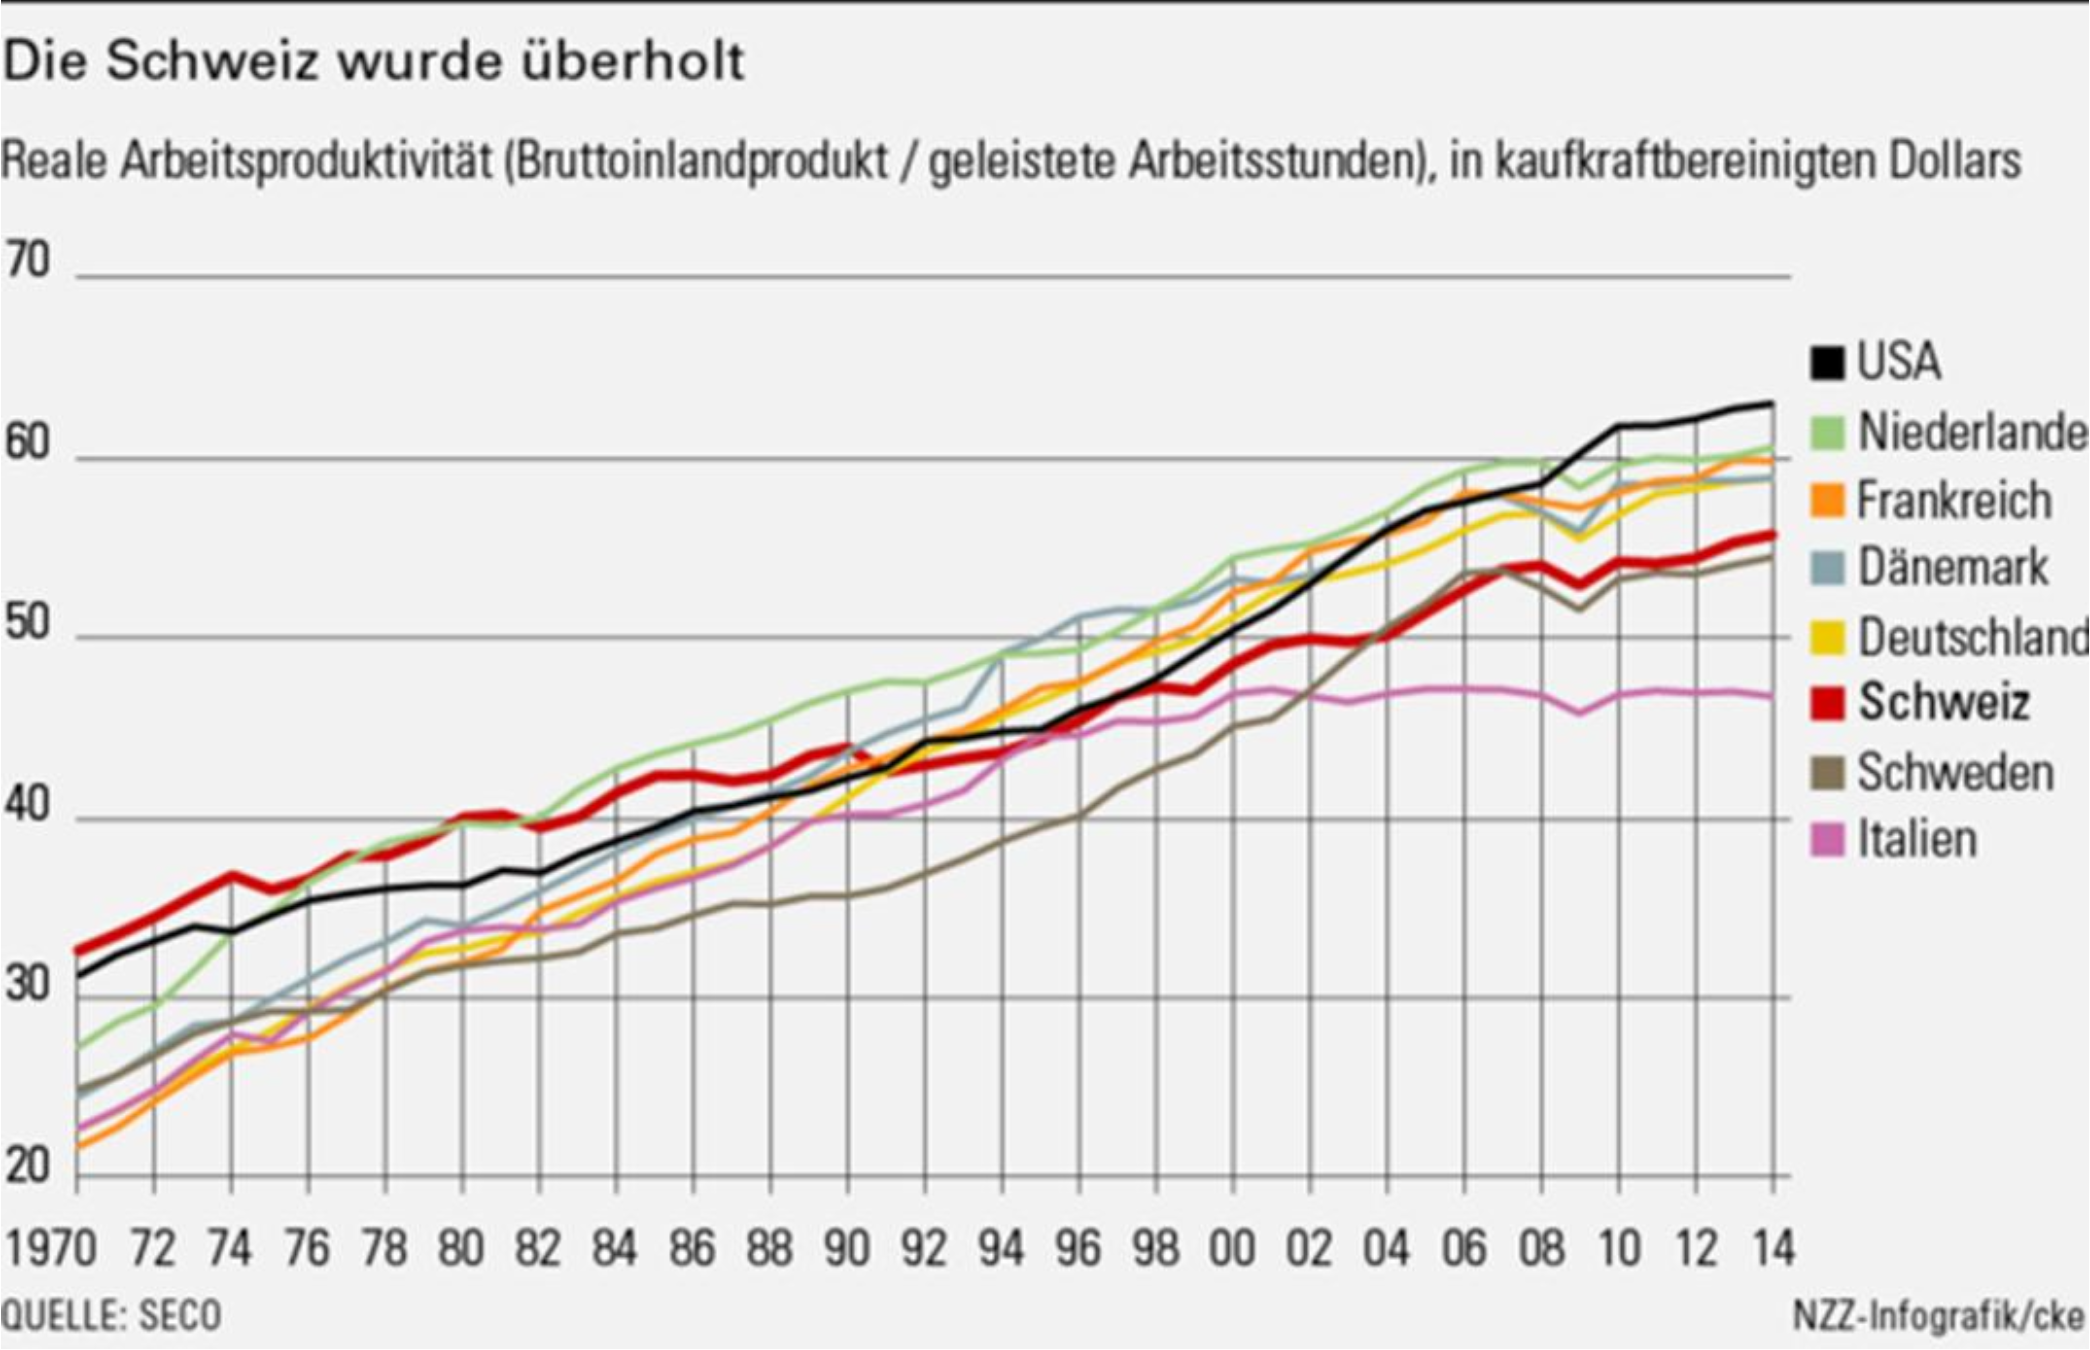
\includegraphics[width=0.8\linewidth]{images/arbeitsproduktivitaet.png}
\end{center}
Produktionsfunktion:
\[
Y = F(K, L, A)
\]

Determinanten:

\begin{itemize}
    \item Mehr Erwerbstätige
    \item Mehr Arbeitsstunden pro Erwerbstätigen
    \item Mehr Realkapital (Investitionen)
    \item Mehr Humankapital (Bildung)
    \item Mehr Know-how (technischer Fortschritt)
\end{itemize}

Langfristig dominiert Produktivitätswachstum.

\begin{center}
    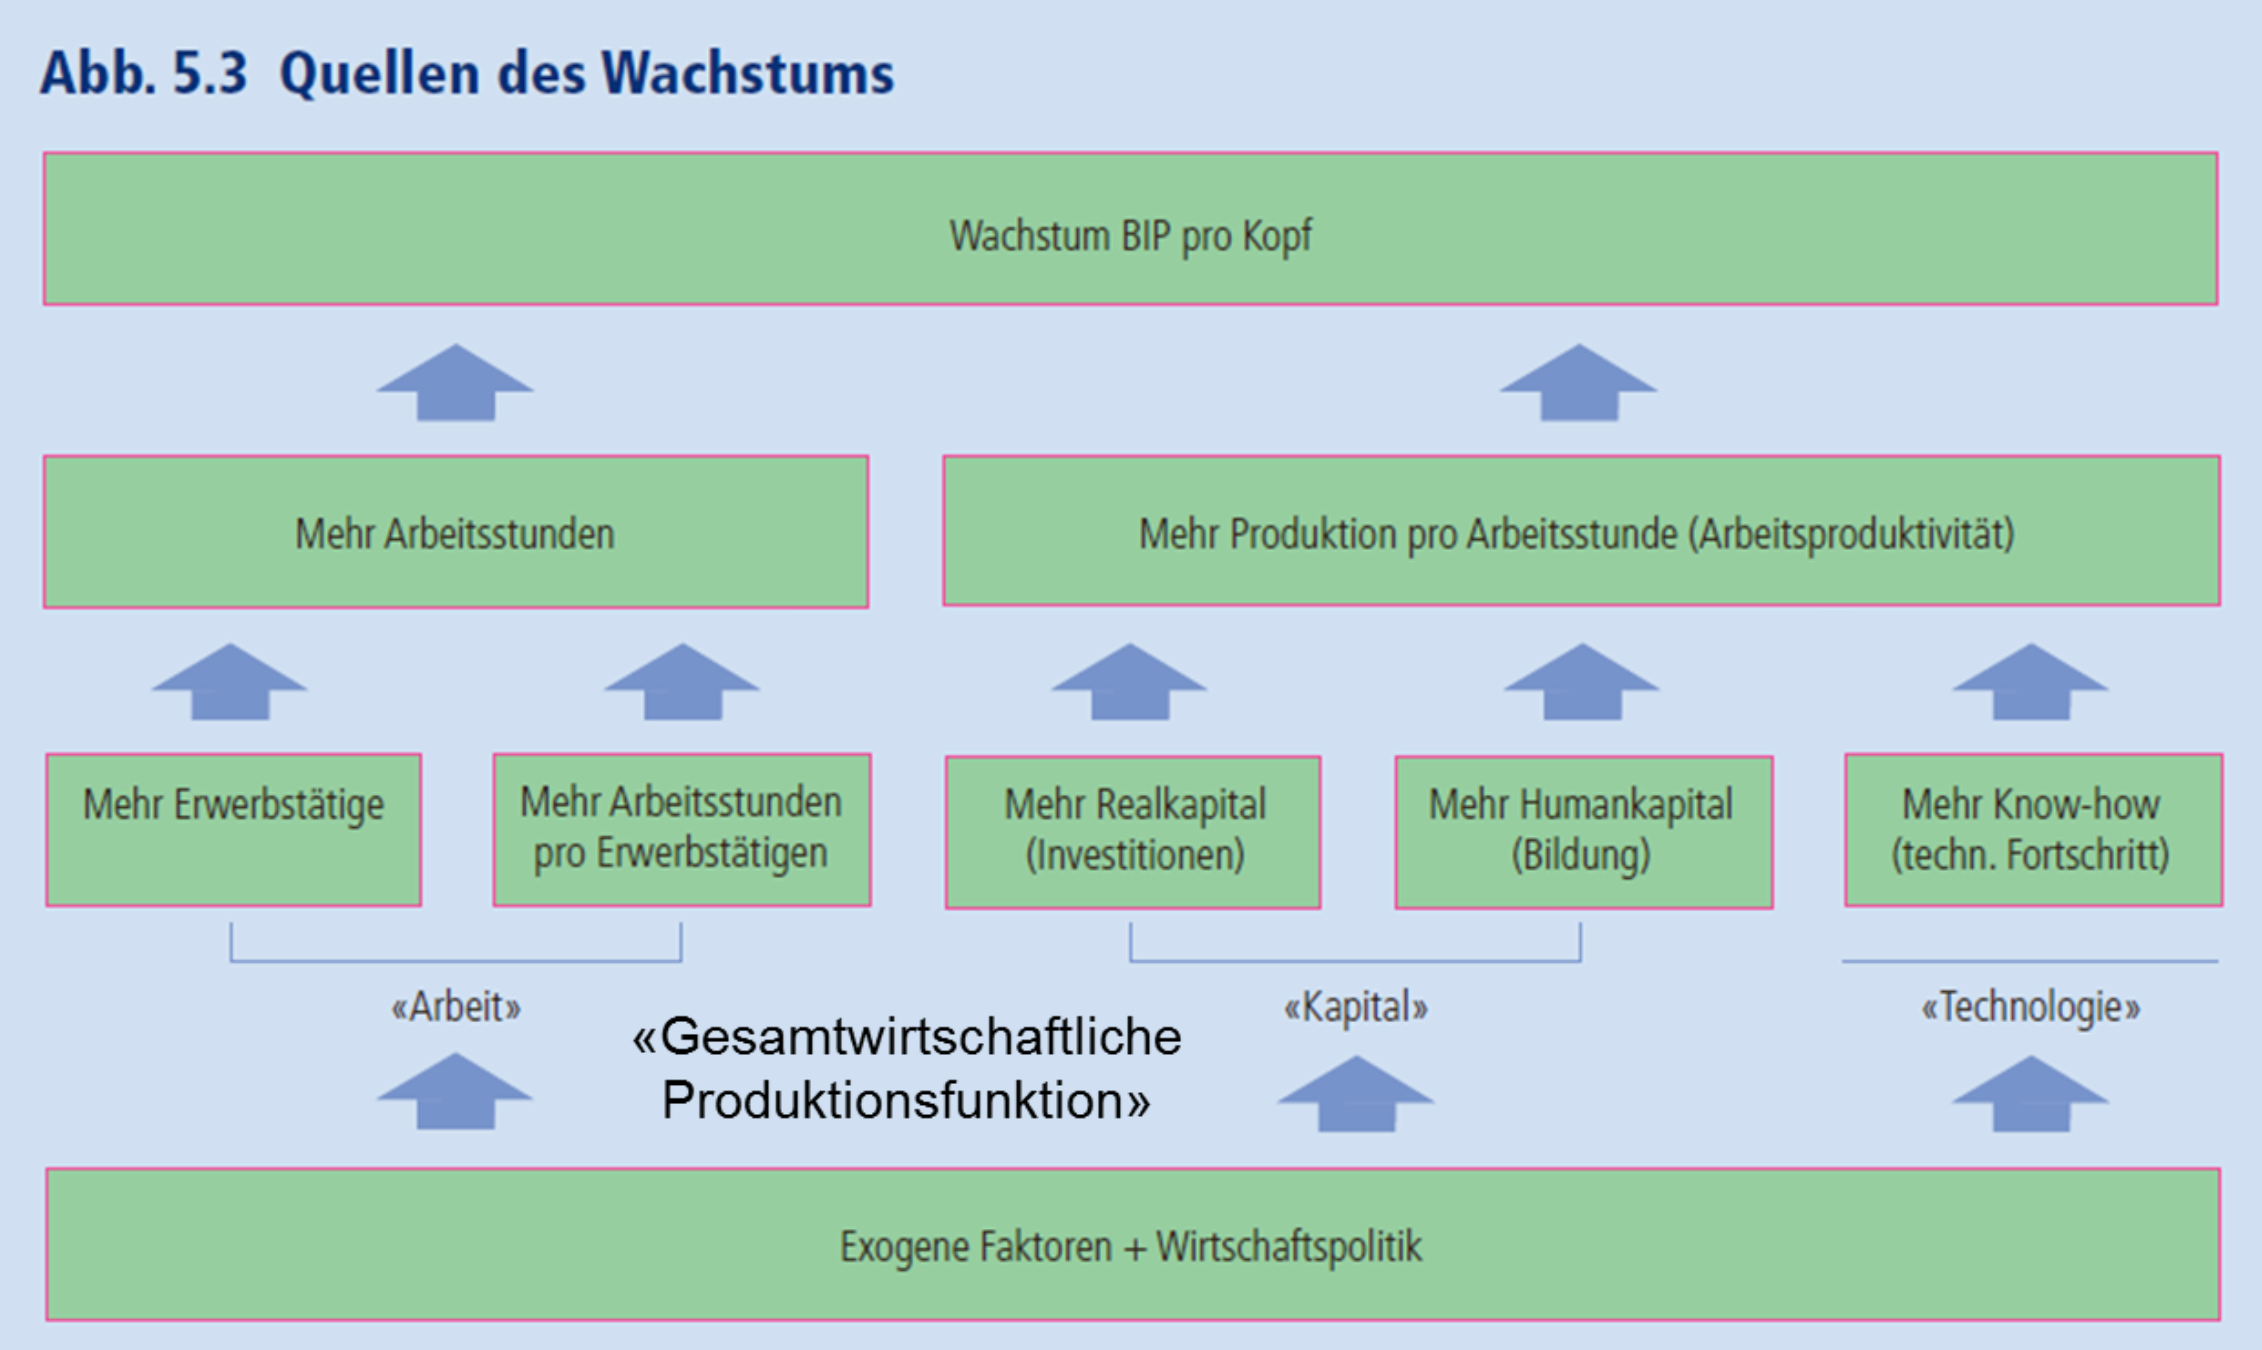
\includegraphics[width=0.8\linewidth]{images/quelle_wachstum.png}
\end{center}

\subsection{Wachstumsentwicklung Schweiz}

Drei historische Phasen:

\begin{itemize}
    \item Phase 1: Moderates Wachstum bis ca. 1950
    \item Phase 2: Starkes Wachstum (Nachkriegsboom)
    \item Phase 3: Deutliche Verlangsamung ab 1970er
\end{itemize}

\begin{center}
    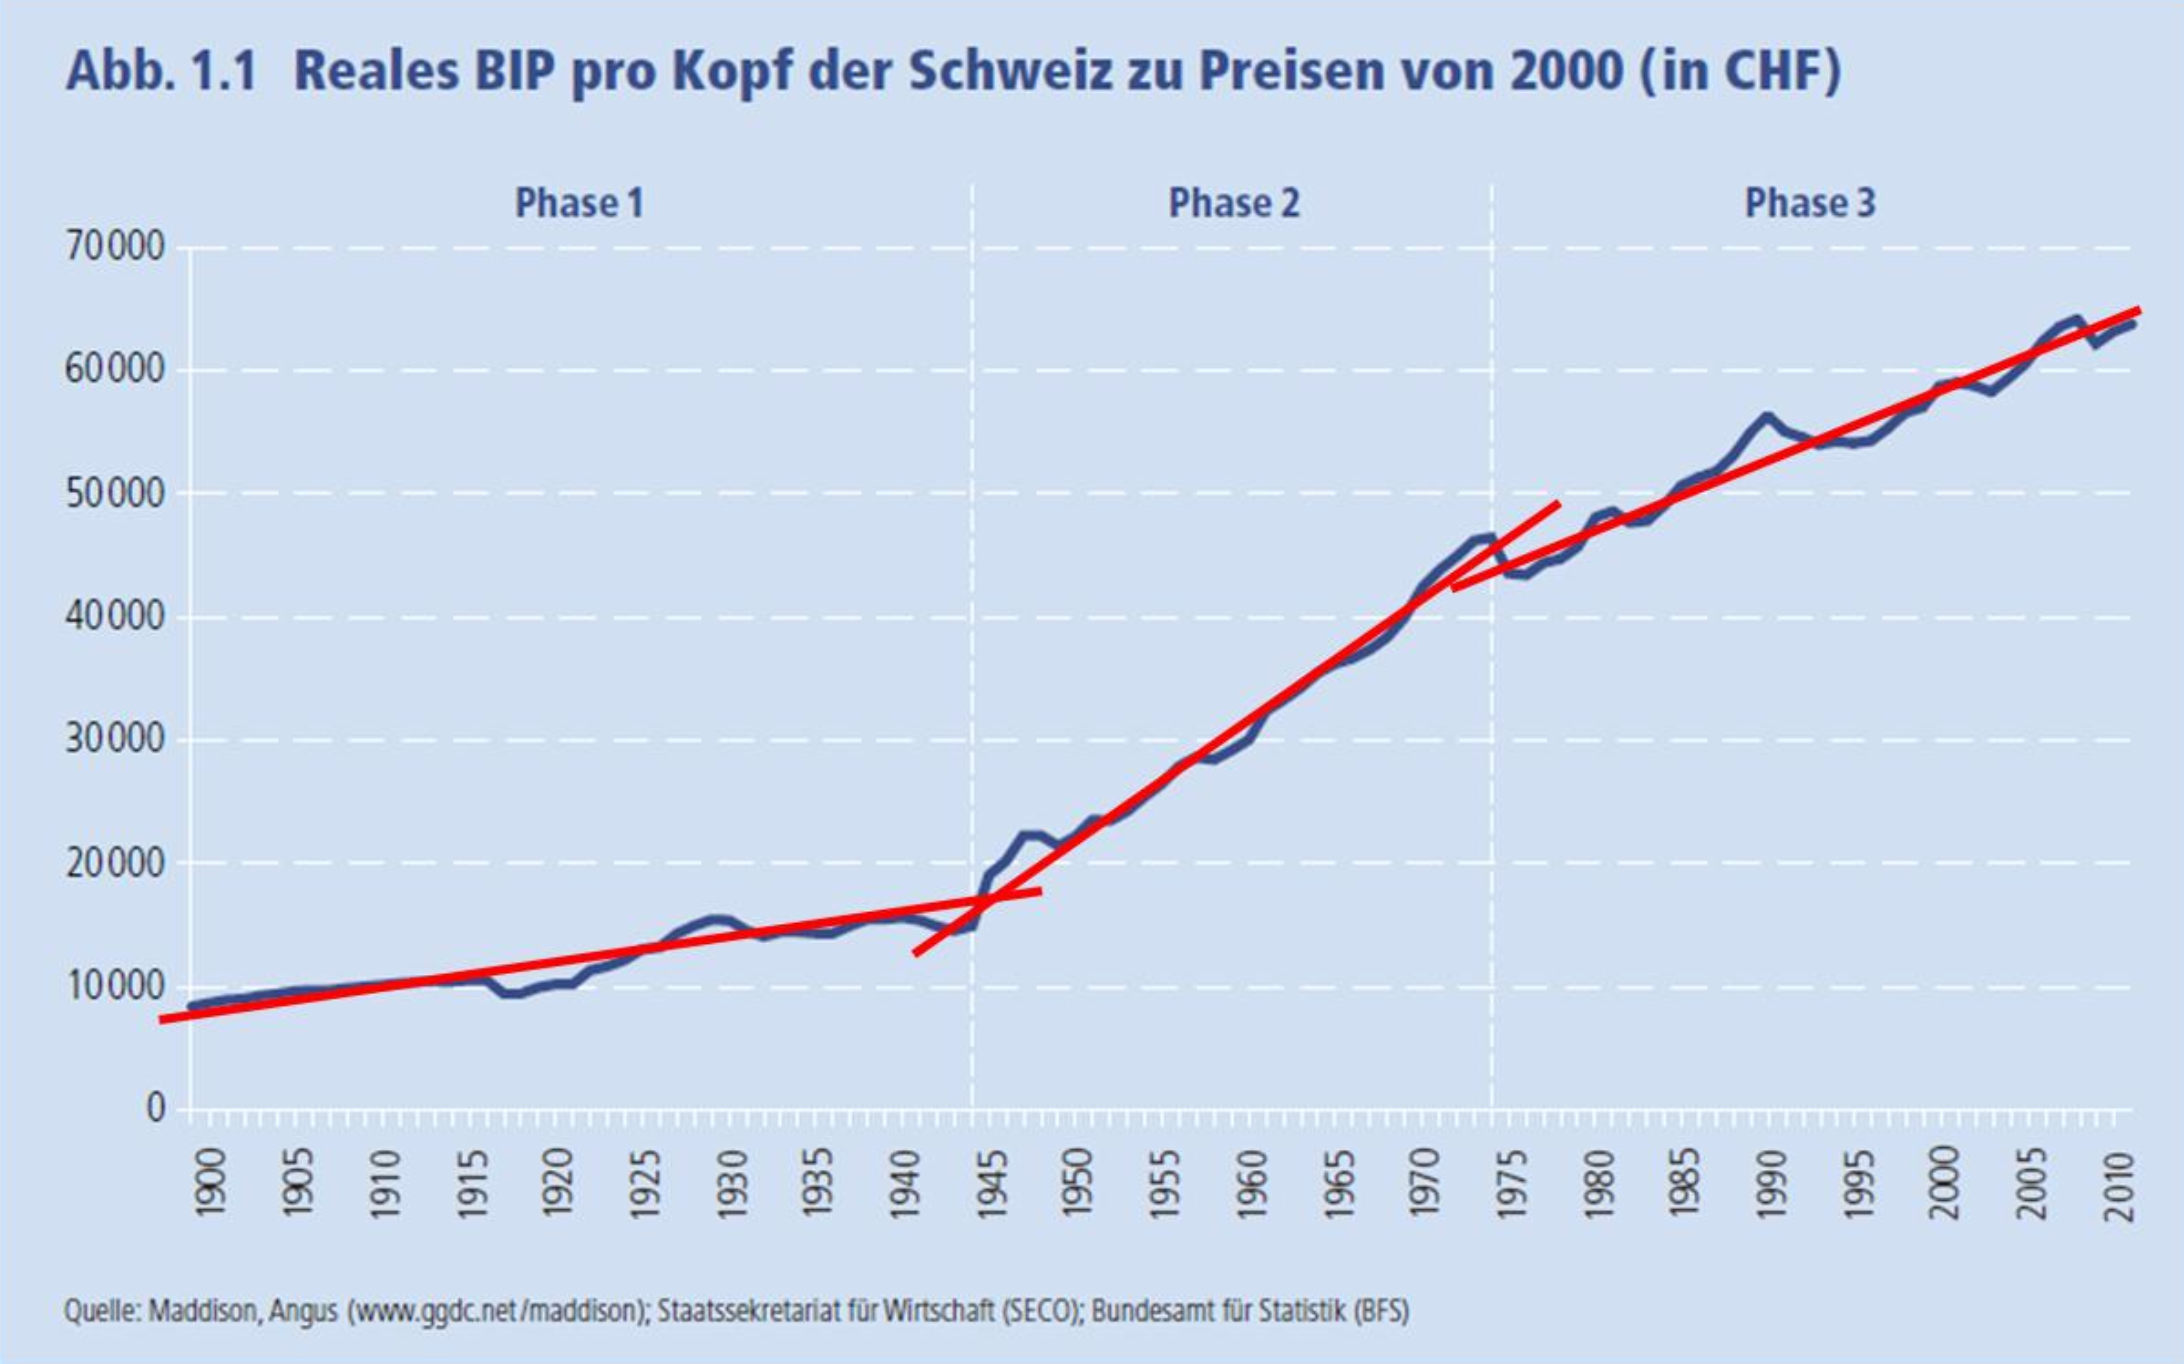
\includegraphics[width=0.8\linewidth]{images/realesbip.png}
\end{center}

Seit den 1990er-Jahren: strukturelle Wachstumsflaute.

\subsection{Diagnose Wachstumsflaute}

Fragestellung:
Liegt die Ursache bei den Arbeitsstunden oder bei der Produktivität?

Analyse zeigt:
Hauptproblem = stagnierendes Produktivitätswachstum.

\subsection{Internationale Produktivitätsvergleiche}

Die Schweiz wurde in Rankings überholt.
Produktivitätswachstum 1995–2014:

\begin{itemize}
    \item Schweiz: ca. 1.2\% pro Jahr
    \item Vergleichsländer teilweise deutlich höher
\end{itemize}

Kleine jährliche Differenzen führen langfristig zu erheblichen Abständen.

\subsection{Mögliche Ursachen der Produktivitätsschwäche}

Die Ursache ist das Wachstum der Staatsquote, insbesondere auch die abschottung des Binnenmarkts( vor allem Landwirtschaft, Energie , Telekommunikation).


\subsection{Rolle der Staatsquote}

These: Expansion staatsnaher Sektoren belastet Produktivitätswachstum.

Beobachtungen:

\begin{itemize}
    \item Starkes Beschäftigungswachstum im öffentlichen Sektor
    \item Geringere Produktivitätsdynamik dort
    \item Auseinanderklaffen von Privat- und Staatssektor
\end{itemize}

Schweiz verliert relativ an internationaler Position.

\subsection{Schweizer Wachstumspolitik ab 2004}

Erste offizielle Wachstumspolitik als Reaktion auf strukturelle Schwäche.

Identifizierte Probleme:

\begin{itemize}
    \item Hochpreisinsel
    \item Überdurchschnittliches Wachstum der Staatsquote
\end{itemize}

\subsection{Wachstumspolitik I (2004–2007)}

Ziele:

\begin{itemize}
    \item Mehr Wettbewerb im Binnenmarkt
    \item Eindämmung Staatsquote
    \item Schuldenbremse
    \item Strukturreformen (Gesundheit, Landwirtschaft, Strom)
    \item Steuerreformen
    \item Administrative Entlastung
\end{itemize}

\subsection{Wachstumspolitik II (2008–2011)}

20 wirtschaftspolitische Massnahmen:

\begin{itemize}
    \item Senkung Kostenniveau
    \item Erhöhung Erwerbsbeteiligung
    \item Stärkung Standortattraktivität
\end{itemize}

\subsection{Wachstumspolitik III (2012–2015)}

Sieben strategische Handlungsfelder:

\begin{itemize}
    \item Binnenmarkt-Wettbewerb
    \item Aussenwirtschaftliche Öffnung
    \item Hohe Erwerbsbeteiligung
    \item Bildung, Forschung, Innovation
    \item Gesunde Staatsfinanzen
    \item Unternehmerfreundliches Recht
    \item Umweltverträglichkeit
\end{itemize}

\subsection{Wachstumspolitik IV (2016–2019)}

Drei Säulen:

\begin{enumerate}
    \item Steigerung Arbeitsproduktivität
    \item Erhöhung wirtschaftlicher Resilienz
    \item Steigerung Ressourcenproduktivität
\end{enumerate}

Zehn konkrete Vorhaben (u.a.):
EU-Bilaterale, Strommarktliberalisierung, Digitalwirtschaft, Energiestrategie 2050, Klimagesetzgebung, Infrastruktur.

Ab 2020 keine neue formelle Initiative.

\subsection{Gesamtfazit der Lerneinheit}

Langfristiges Wachstum ist zentraler Treiber des Wohlstands.

Die Schweizer Wachstumsproblematik ist primär ein Produktivitätsproblem.

Wachstumspolitik adressiert strukturelle Rahmenbedingungen:
Wettbewerb, Innovation, Bildung, Staatsfinanzen, Marktöffnung.

Konjunkturpolitik ist kurzfristig relevant –
Wachstumspolitik ist strategisch entscheidend.

    \end{layout}
\end{document}
